\chapter{Virtualización}

\section{Qué es la virtualización}

La virtualización es la creación de una versión virtual basada en software de algo, en lugar de una física. Se puede aplicar a sistemas operativos, almacenamiento, servidores, aplicaciones, redes… y es una manera de reducir gastos, aumentar eficiencia y agilidad en las empresas.  

\subsection{Tipos de virtualización}

Estos son los 4 tipos de virtualización más habituales.
\subsubsection{Virtualización de servidores}

La virtualización en servidores ayuda a evitar ineficiencias ya que permite ejecutar varios sistemas operativos en una máquina física como máquinas virtuales, con acceso a los recursos de todos. 
También permite generar un cluster de servidores en un único recurso para así mejorar mucho más la eficiencia y la reducción de costes. También permite el aumento de rendimiento de las aplicaciones, la disponibilidad al aumentar la velocidad en la carga de trabajo.

\subsubsection{Virtualización de escritorios}

La implementación de escritorios virtualizados permite ofrecer a las sucursales o empleados externos… de forma rápida y sencilla un entorno de trabajo y una reducción de la inversión a la hora de gestionar cambios en estos. 

\subsubsection{Virtualización de red}

Se trata de reproducir una red completa física mediante software, para poder ejecutar los mismo servicios que una red convencional y dispositivos. Cuentan con las misma características y garantías que las redes físicas con las ventajas que nos ofrece la virtualización más la liberación del hardware.

\subsubsection{Almacenamiento definido por software}

La virtualización del almacenamiento permite prescindir de  los discos de los servidores, los combina en depósitos de almacenamiento de alto rendimiento y los distribuye como software. Este nuevo modelo es permite aumentar la eficiencia en el guardado de datos.
\pagebreak  

\subsection{Ventajas de la virtualización}

Como se ha podido apreciar en los tipos de virtualización, esta conlleva una mejora considerable tanto en el rendimiento, agilidad, flexibilidad, escalabilidad… Como en una reducción de costes considerables tanto en tiempo como monetarios y una simplificación en la gestión de la infraestructura.

\begin{itemize}
\item Reduce los costes de capital y los gastos operativos.
\item Minimiza o elimina los tiempos de inactividad.
\item Aumenta la productividad, la eficiencia, la agilidad y la capacidad de respuesta.
\item Implementa aplicaciones y recursos con más rapidez.
\item Garantiza la continuidad del negocio y la recuperación ante desastres.
\item Simplifica la gestión del centro de datos. 
\end{itemize}

\section{Qué es Docker}

Docker es un proyecto Open Source basado en contenedores de Linux, es básicamente un motor de contenedores que usa características del Kernel de Linux.

La idea detrás de Docker es crear contenedores ligeros y portables para las aplicaciones software que puedan ejecutarse en cualquier máquina con Docker instalado,
independientemente del sistema operativo que la máquina tenga por debajo, facilitando así también los despliegues.

De una manera más sencilla Docker los que nos proporciona es la opción de poder meter en pequeños contenedores todo aquello que nuestra aplicación necesite y poder desplegarla en cualquier maquina que tenga instalado Docker sin preocuparnos de nada más. 

Se podría decir que son pequeñas “máquinas virtuales” pero muchos más ligeras ya que utilizan el sistema operativo de donde se ejecuta y el contenido relevante para ejecutar la aplicación está dentro de los contenedores.
\newline 

Docker es:

\begin{itemize}
\item Open-Source para la gestión de "virtualización de contenedores"
\item Aísla múltiples sistemas de archivos en el interior del mismo host
\begin{itemize}
\item Las instancias se llaman Contenedores
\item Te dan la ilusión de estar dentro de una máquina virtual
\end{itemize}
\item Piensa en entornos de ejecución o "sandboxes"
\item No hay necesidad de un hypervisor (rápido de ejecutar)
\item Requiere x64 y Linux kernel 3.8+
\end{itemize}
\pagebreak 
Docker no es:

\begin{itemize}
\item Un lenguaje de programación
\item Un sistema operativo
\item Una máquina virtual
\item Una imagen en el concepto tradicional de la máquina virtual basada en hipervisor
\end{itemize}

\section{Máquinas Virtuales vs Docker}

Las máquinas virtuales, incluyen toda la aplicación, los binarios y librerías necesarias, y todo un sistema operativo cosa que hace que que ocupen mucho espacio, el tiempo de ejecución sea lento, la necesidad de un Hipervisor para su utilización.

Por lo contrario Docker container incluyen la aplicación y todas sus dependencias pero comparten el núcleo con otros contenedores, funcionando como procesos aislados en el sistema de ficheros del sistema operativo. Docker container no están vinculados a ninguna infraestructura específica: se ejecutan en cualquier ordenador, en cualquier infraestructura, y en cualquier cloud.

\begin{figure}[htb]
\begin{center}
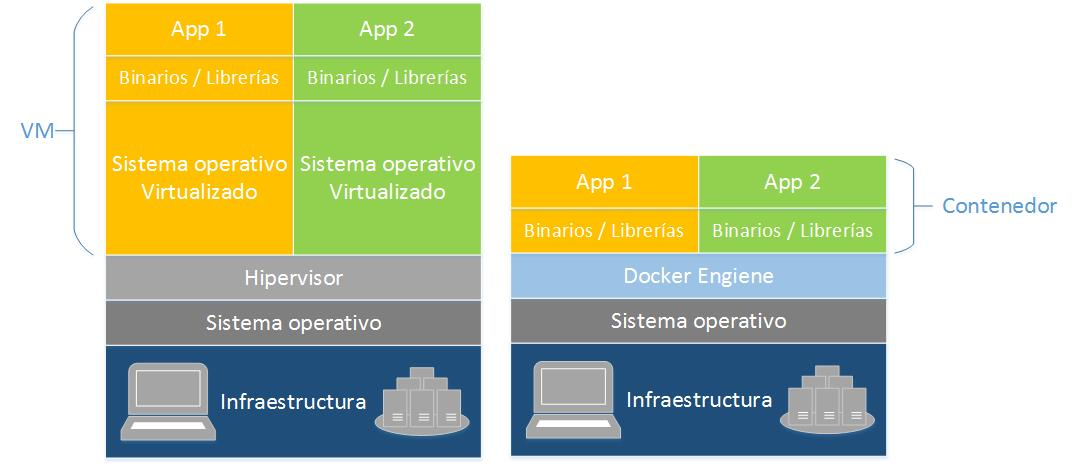
\includegraphics[width=1\textwidth]{./setup/VrvsDocker}
\caption{Comparativa de máquina virtual y Docker}
\label{Vs:VrvsDocker}
\end{center}
\end{figure}

En la imagen \ref{Vs:VrvsDocker} se puede ver las diferencias comentadas anteriormente, mientras la primera columna sería la virtualización de 2 aplicaciones se puede dectectar que está la capa intermedia del Hipervisor el cual nos permite ejecutar los sistemas operativos virtualizados, todos los binarios y librerías que requieren cada aplicación y finalmente la aplicación. 
En la segunda columna tenemos la contenerización de 2 aplicaciones, podemos observar que no hace falta un hipervisor ya que utilizan el sistema operativo de la infraestructura donde se ejecuta, pero si son necesarios los binarios y las librerías.
A simple vista se puede apreciar que si eliminamos el sistema operativo la infraestructura completa se hace más liviana y rápida de ejecutar.

\section{Porque Docker?}

Por lo motivos listados en el apartados anteriores se decidió en utilizar Docker para realizar el despliegue de las aplicaciones, ya que se necesita de una tecnología la cual pueda ser almacenada en dispositivos con una memoria reducida en este caso docker la cumple. 

Su rapidez a la hora de levantar el servicio, en el mundo de IoT el tiempo es un bien preciado y los sistemas se pueden apagar y encender constantemente para evitar gastos de energía innecesarios.

La facilidad para poder desplegar los servicios, con Docker desplegar servicios es muy sencillo solo requiere tenerlo instalado y ejecutar el contenedor para que el servicio esté activo.

La sencillez a la hora de mantener el sistema, si hay que hacer actualizaciones o controles de una pequeña parte del servicio solo habria que cambiar o actualizar ese contenedor no todo el sistema. Esto es un gran ahorro en recursos y tiempo. 

Por todo esto se piensa que Docker puede ser una buena tecnología para desplegar sistemas de Iot. También se tiene en cuenta que la utilización de una Raspberry 3 no es un aparato con unas capacidades limitadas como podría ser un sensor utilizado normalmente pero si que puede validar todas las funciones listadas anteriormente y servir como preámbulo para la utilización en el resto de despliegues.  

\section{Cómo funciona Docker?}

En este punto se explicara brevemente aspectos de la arquitectura, funcionamiento y puesta en marcha de Docker.  

\subsection{Arquitectura}

Docker usa una arquitectura cliente-servidor. El cliente de Docker se comunica con el Daemon de Docker para crear, ejecutar y distribuir los contenedores. El cliente como el Daemon puede estar en el mismo sistema o poder conectarte remotamente.
Como Docker usa el kernel de linux para su ejecución si el sistema operativo del sistema no es este se deberá usar una pequeña capa extra en la arquitectura la cual sería una VM (boot Docker) para poder correr docker en la máquina. 

\subsubsection{Cliente de Docker}

Es la principal interfaz de usuario para docker, acepta los comandos del usuario y se comunica con el daemon de docker.

\subsubsection{Imágenes de Docker (Docker Images)}

Las imágenes de Docker son plantillas de solo lectura, que nos permitirá crear contenedores basados en su configuración.

\subsubsection{Registros de Docker (Docker Registries)}

Los registros de Docker guardan las imágenes, estos son repos públicos o privados donde podemos subir o descargar imágenes. Sería similar a GitHub para imágenes de docker (Docker Hub).

\subsubsection{Contenedores de Docker (Docker Containers)}

El contenedor de docker contiene todo lo necesario para ejecutar una aplicación. Cada contenedor se crea de una imagen de docker y es una plataforma aislada.
\newline

En la figura \ref{Inf:Infraestructura} podemos apreciar gráficamente cómo sería la arquitectura básica. 

El cliente podría hacer los comandos básicos de docker:

\texttt{Docker Build}: Hace un build de un DockerFile y generar una imagen de docker, en la figura está representado siguiendo las flechas rojas en la cual podemos ver que el cliente se comunica con el Daemon y este genera la imagen. 

\texttt{Docker Pull}: El cual nos permite descargar una imagen de los repositorios de Docker, en la imagen se puede observar siguiendo las flechas verdes. Que igual que el comando anterior se comunica el cliente con el Daemon para que este proceda a hacer la descarga de la imagen del repositorio. 

\texttt{Docker Run}: Ejecuta una imagen para generar un contendor de esta. Si seguimos las flechas azules, veremos como nuevamente el cliente al ejecutar esa comanda se comunica con el Daemon este busca la imagen a la cual se le quiere hacer ejecutar y se levanta un contenedor con la configuración de la imagen.

\begin{figure}[htb]
\begin{center}
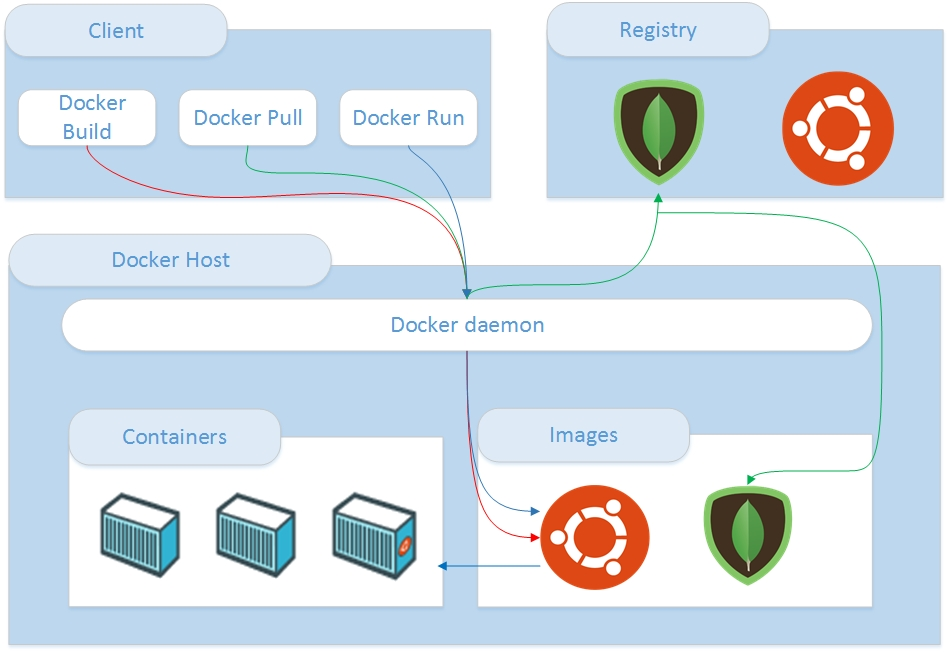
\includegraphics[width=0.90\textwidth]{./setup/Infraestructura}
\caption{Infraestructura de Docker}
\label{Inf:Infraestructura}
\end{center}
\end{figure}

\subsection{Creacion de Imagenes}

Como se comentó en el punto anterior las imágenes de docker son las plantillas para poder levantar los contenedores, por eso la importancia de saber crear imágenes y personalizarlas ya que solo permiten lectura y los cambios que hagamos en los contenedores no se verán reflejados en estas.

La manera más sencilla de crear una imagen es descargarla del Docker Hub con el comando explicado con anterioridad:

\begin{center}
\texttt{docker pull [OPTIONS] NAME[:TAG|@DIGEST]}
\end{center}

Este comando nos permite descargar una imagen en una versión concreta o tag dependiendo de nuestras necesidades, por defecto si no se pone nada descargara la ultima. 

\begin{center}
\texttt{FOTO DE HACER UN PULL Y DEL DOCKER IMAGES}
\end{center}

En las figuras XX podemos apreciar como se descarga la última versión de la imagen de mongo y nos genera esta imagen. 

Una vez tenemos la imagen pasaremos a levantar el contenedor para poder ejecutar el servicio con otro de los comandos explicados. 

\begin{center}
\texttt{docker run [OPTIONS] IMAGE [COMMAND] [ARG...]}
\end{center}

En las figuras se puede apreciar cómo utilizando el comando \texttt{docker ps} que nos permite ver que contenedores están levantados. No hay ninguno y al inicializar con el comando \texttt{docker run mongo} nos levanta el servicio y esta vez si aparece el contenedor.
\newline

La segunda manera de crear y personalizar imágenes es mediante un \texttt{DockerFile}, que es un documento de texto donde se encuentra todos los comandos que se deben ejecutar para generar nuestra imagen.

El comando \texttt{docker build} comunica al daemon de docker que debe de leer el \texttt{DockerFile} del directorio actual y seguir las instrucciones línea por línea para la creación de nuestra imagen. Este proceso se va pintando los resultados por pantalla y generando imágenes intermedias para obtener así una cache que nos permitirá en caso de errores, una vez corregido el DockerFile, continuar desde el punto conflictivo y no compilarlo todo de nuevo. 

\begin{center}
\texttt{Explicacioens de la imagen del dockerfile}
\end{center}

\subsection{Docker Compose}

Docker Compose es un orquestador que nos permite ejecutar aplicaciones que utilicen varios contenedores a la vez.
Se creará un archivo docker-compose.yml donde se configurar todos los servicios necesarios para nuestra aplicación. Una vez ejecutado este archivo nos generará todas las imágenes y con estas los contenedores especificados a la vez que arrancará la aplicación.
\pagebreak

Los comandos que se utilizarán serán similares a los utilizados en la creación de imágenes.

\begin{center}
\texttt{docker-compose up}
\end{center} 

Permite ejecutar el servicio y se nos levante todos los contenedores.

\begin{center}
\texttt{docker-compose stop}
\end{center} 

Detendrá el servicio y detener los contenedores. 
\newline

Docker-compose también nos permite ejecutar solo partes del.yml para levantar solo algunos de los contenedores igual que detener solo algunos de ellos, pasándole por parámetro el nombre del contenedor. 
\begin{center}
\begin{verbatim}
version: '2'
services:
 mongo:
  container_name: mongo
  restart: always
  image: partlab/ubuntu-arm-mongodb
  volumes:
   - mongo-data:/data/db
  command: /usr/bin/mongod --smallfiles --journal
 aaaida:
  container_name: aaaidaArm
  restart: always
  image: alteraid/aaaida-datastore-arm
  links:
   - mongo:mongo 
  environment:
   - NODE_ENV=docker
  ports:
   - "40000:40000"
volumes:
 mongo-data:
   driver: local
\end{verbatim}
\end{center} 
